\begin{figure}[tb] % *!
    \centering
    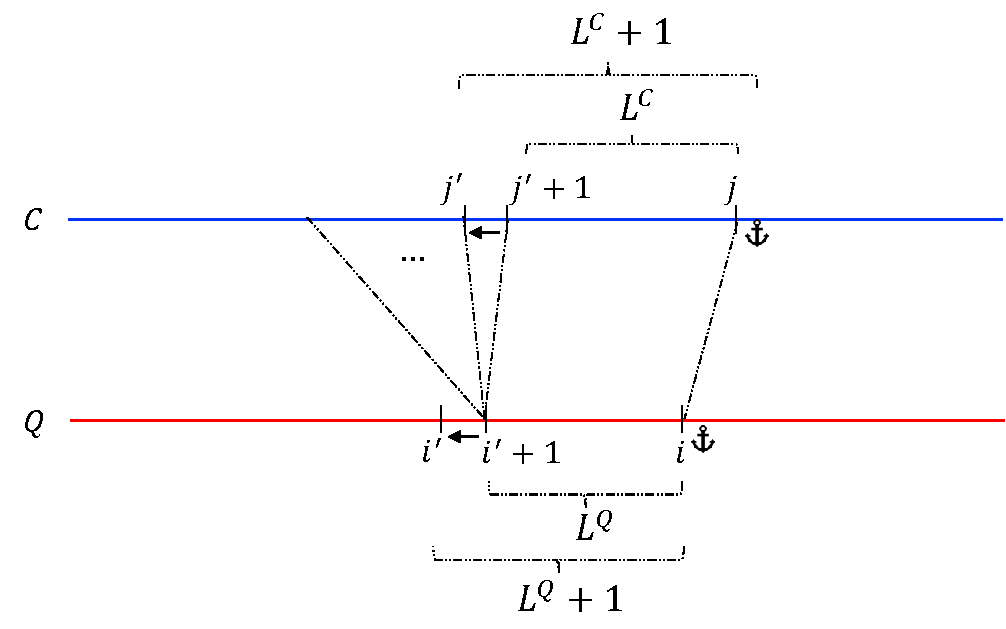
\includegraphics[width=1.0\columnwidth]{figures/L_Q-L_C-relationship.pptx.pdf}
    \caption{
    $L^Q$ and $L^C$ are the lengths of the considered segments of $Q$ and $C$, respectively.
    The anchor signs indicate that the segment ends are fixed.
    The lengths increase as the starting indices decrease.
    The same segment of length $L^Q$ is first compared with a set of lengthening $C$ segments, where the starting index is decreased by $1$ at each iteration.
    After that, the length of the $Q$ segment is increased by $1$.
    }
    \label{fig:L_Q-L_C-relationship}
\end{figure}